\documentclass[border=10pt,margin=5pt,tikz,dvisvgm,rgb,utf8]{standalone}
\usepackage{ctex,xeCJK}  % 中文环境
\setCJKmainfont[BoldFont=Source Han Sans SC]{Source Han Serif SC}
\usepackage{calc,fontawesome,forest,smartdiagram,xcolor}
\usetikzlibrary{animations,arrows,automata,graphs,matrix,positioning,shadows,shapes}

\begin{document}
\renewcommand{\baselinestretch}{0.4}

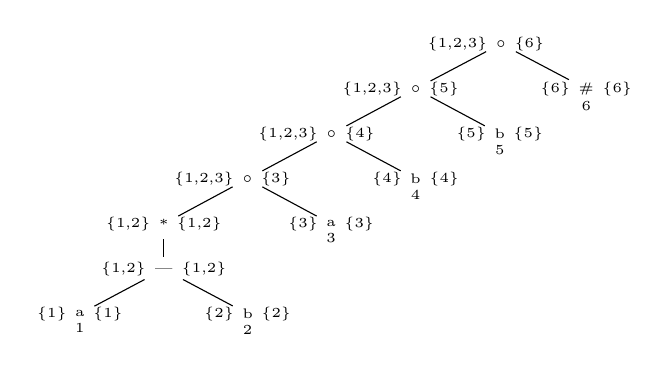
\begin{tikzpicture}
  \node[](1){\tiny a};
  \node[right=5em of 1](2){\tiny b};
  \node[above=1.15em of $(1)!0.5!(2)$](A){\tiny |};
  \node[above=0.64em of A](B){\tiny *};
  \node[right=5em of B](3){\tiny a};
  \node[above=1.15em of $(B)!0.5!(3)$](C){\tiny $\circ$};
  \node[right=5em of C](4){\tiny b};
  \node[above=1.15em of $(C)!0.5!(4)$](D){\tiny $\circ$};
  \node[right=5em of D](5){\tiny b};
  \node[above=1.15em of $(D)!0.5!(5)$](E){\tiny $\circ$};
  \node[right=5em of E](6){\tiny \#};
  \node[above=1.15em of $(E)!0.5!(6)$](F){\tiny $\circ$};

  \node[below=-0.45em of 1](_1){\tiny 1};
  \node[below=-0.45em of 2](_2){\tiny 2};
  \node[below=-0.45em of 3](_3){\tiny 3};
  \node[below=-0.45em of 4](_4){\tiny 4};
  \node[below=-0.45em of 5](_5){\tiny 5};
  \node[below=-0.45em of 6](_6){\tiny 6};

  \path[-]
  (1) edge (A)
  (2) edge (A)
  (A) edge (B)
  (B) edge (C)
  (3) edge (C)
  (C) edge (D)
  (4) edge (D)
  (D) edge (E)
  (5) edge (E)
  (E) edge (F)
  (6) edge (F);

  \node[left=-0.4em of 1](first_1){\tiny \{1\}};
  \node[right=-0.4em of 1](last_1){\tiny \{1\}};
  \node[left=-0.4em of 2](first_2){\tiny \{2\}};
  \node[right=-0.4em of 2](last_2){\tiny \{2\}};
  \node[left=-0.4em of A](first_A){\tiny \{1,2\}};
  \node[right=-0.4em of A](last_A){\tiny \{1,2\}};
  \node[left=-0.4em of B](first_B){\tiny \{1,2\}};
  \node[right=-0.4em of B](last_B){\tiny \{1,2\}};
  \node[left=-0.4em of 3](first_3){\tiny \{3\}};
  \node[right=-0.4em of 3](last_3){\tiny \{3\}};
  \node[left=-0.4em of C](first_C){\tiny \{1,2,3\}};
  \node[right=-0.4em of C](last_C){\tiny \{3\}};
  \node[left=-0.4em of 4](first_4){\tiny \{4\}};
  \node[right=-0.4em of 4](last_4){\tiny \{4\}};
  \node[left=-0.4em of D](first_D){\tiny \{1,2,3\}};
  \node[right=-0.4em of D](last_D){\tiny \{4\}};
  \node[left=-0.4em of 5](first_5){\tiny \{5\}};
  \node[right=-0.4em of 5](last_5){\tiny \{5\}};
  \node[left=-0.4em of E](first_E){\tiny \{1,2,3\}};
  \node[right=-0.4em of E](last_E){\tiny \{5\}};
  \node[left=-0.4em of 6](first_6){\tiny \{6\}};
  \node[right=-0.4em of 6](last_6){\tiny \{6\}};
  \node[left=-0.4em of F](first_F){\tiny \{1,2,3\}};
  \node[right=-0.4em of F](last_F){\tiny \{6\}};

\end{tikzpicture}

\end{document}
